\documentclass[tikz,border=10pt]{standalone}
\usepackage{tikz}
\usepackage{amsmath}
\usepackage{amsfonts}
\usetikzlibrary{arrows.meta,positioning,shapes.geometric,shapes.misc,fit,backgrounds,calc,decorations.pathreplacing,patterns}

\begin{document}
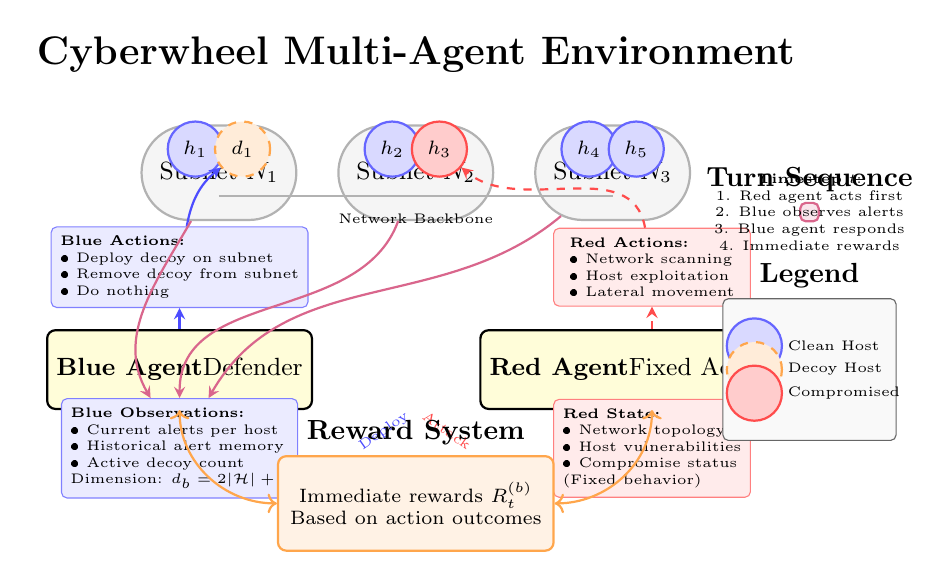
\begin{tikzpicture}[
    % Clean, organized node styles
    host/.style={circle, draw=blue!60, fill=blue!15, minimum size=7mm, font=\scriptsize, thick},
    decoy/.style={circle, draw=orange!70, fill=orange!15, minimum size=7mm, font=\scriptsize, thick, dashed},
    compromised/.style={circle, draw=red!70, fill=red!20, minimum size=7mm, font=\scriptsize, thick},
    subnet/.style={rounded rectangle, draw=gray!60, fill=gray!8, minimum width=22mm, minimum height=12mm, font=\small, thick},
    agent/.style={rectangle, draw=black, fill=yellow!15, minimum width=18mm, minimum height=10mm, font=\small, rounded corners=3pt, thick},
    infobox/.style={rectangle, draw=gray!50, fill=gray!5, rounded corners=2pt, font=\tiny, align=left, minimum width=25mm},
    action/.style={->, thick, blue!70, >=stealth},
    attack/.style={->, thick, red!70, dashed, >=stealth},
    flow/.style={->, thick, purple!60, >=stealth}
]

% Title
\node[font=\Large\bfseries] at (0, 4.5) {Cyberwheel Multi-Agent Environment};

% Network Layer (Top)
\node[subnet] (subnet1) at (-2.5, 3) {Subnet $N_1$};
\node[subnet] (subnet2) at (0, 3) {Subnet $N_2$};  
\node[subnet] (subnet3) at (2.5, 3) {Subnet $N_3$};

% Hosts within subnets - cleaner positioning
\node[host] (h1) at (-2.8, 3.3) {$h_1$};
\node[decoy] (d1) at (-2.2, 3.3) {$d_1$};

\node[host] (h2) at (-0.3, 3.3) {$h_2$};
\node[compromised] (h3) at (0.3, 3.3) {$h_3$};

\node[host] (h4) at (2.2, 3.3) {$h_4$};
\node[host] (h5) at (2.8, 3.3) {$h_5$};

% Network connections (simplified)
\draw[gray!60, thick] (-2.5, 2.7) -- (0, 2.7) -- (2.5, 2.7);
\node[below, font=\tiny] at (0, 2.6) {Network Backbone};

% Agent Layer (Bottom)  
\node[agent] (blue_agent) at (-3, 0.5) {\textbf{Blue Agent}\\Defender};
\node[agent] (red_agent) at (3, 0.5) {\textbf{Red Agent}\\Fixed Adversary};

% Clean action representation
\node[infobox, draw=blue!50, fill=blue!8] (blue_actions) at (-3, 1.8) {
    \textbf{Blue Actions:}\\
    • Deploy decoy on subnet\\
    • Remove decoy from subnet\\
    • Do nothing
};

\node[infobox, draw=red!50, fill=red!8] (red_actions) at (3, 1.8) {
    \textbf{Red Actions:}\\
    • Network scanning\\
    • Host exploitation\\
    • Lateral movement
};

% State information
\node[infobox, draw=blue!50, fill=blue!8] (blue_state) at (-3, -0.5) {
    \textbf{Blue Observations:}\\
    • Current alerts per host\\
    • Historical alert memory\\
    • Active decoy count\\
    Dimension: $d_b = 2|\mathcal{H}| + 2$
};

\node[infobox, draw=red!50, fill=red!8] (red_state) at (3, -0.5) {
    \textbf{Red State:}\\
    • Network topology\\
    • Host vulnerabilities\\
    • Compromise status\\
    (Fixed behavior)
};

% Clean flow arrows
\draw[action] (blue_agent) -- (blue_actions);
\draw[action] (blue_actions) to[out=80, in=220] (d1) node[midway, left, font=\tiny, rotate=35] {Deploy};

\draw[attack] (red_agent) -- (red_actions);  
\draw[attack] (red_actions) to[out=100, in=320] (h3) node[midway, right, font=\tiny, rotate=-35] {Attack};

% Observation flows
\draw[flow] (subnet1) to[out=240, in=120] (blue_state);
\draw[flow] (subnet2) to[out=250, in=90] (blue_state);
\draw[flow] (subnet3) to[out=220, in=60] (blue_state);

% Reward system (centralized)
\node[rectangle, draw=orange!70, fill=orange!10, minimum width=35mm, minimum height=12mm, rounded corners=3pt, thick] (reward) at (0, -1.2) {};
\node[above] at (reward.north) {\textbf{Reward System}};
\node[font=\scriptsize, align=center] at (reward.center) {
    Immediate rewards $R_t^{(b)}$\\
    Based on action outcomes
};

\draw[<->, orange!70, thick] (blue_agent) to[out=270, in=180] (reward);
\draw[<->, orange!70, thick] (red_agent) to[out=270, in=0] (reward);

% Turn sequence (top right)
\node[rectangle, draw=purple!60, fill=purple!10, rounded corners=2pt, thick] (sequence) at (5, 2.5) {};
\node[above] at (sequence.north) {\textbf{Turn Sequence}};
\node[font=\tiny, align=center] at (sequence.center) {
    \textbf{Timestep} $t$:\\
    1. Red agent acts first\\
    2. Blue observes alerts\\
    3. Blue agent responds\\
    4. Immediate rewards
};

% Legend (bottom right)
\node[rectangle, draw=black!60, fill=gray!5, minimum width=22mm, minimum height=18mm, rounded corners=2pt] (legend) at (5, 0.5) {};
\node[above] at (legend.north) {\textbf{Legend}};
\node[host] at (4.3, 0.8) {};
\node[right, font=\tiny] at (4.6, 0.8) {Clean Host};
\node[decoy] at (4.3, 0.5) {};
\node[right, font=\tiny] at (4.6, 0.5) {Decoy Host};
\node[compromised] at (4.3, 0.2) {};
\node[right, font=\tiny] at (4.6, 0.2) {Compromised};

\end{tikzpicture}
\end{document}